\documentclass{article}

%Aus dem LaTex Template der Universit�t Stuttgart
%------------------------------------------------
\usepackage[utf8]{inputenc}
\usepackage[T1]{fontenc}
\usepackage[sfdefault]{ClearSans} %% option 'sfdefault' activates Clear Sans as the default text font
\usepackage{cmap}
\usepackage[ngerman]{babel}
\usepackage{graphicx}
\usepackage[pdftex,hyperref,dvipsnames]{xcolor}
\usepackage{listings}
\usepackage[a4paper,lmargin={2cm},rmargin={2cm},tmargin={3.5cm},bmargin = {2.5cm},headheight = {4cm}]{geometry}
\usepackage{amsmath,amssymb,amstext,amsthm}
\usepackage[lined,algonl,boxed]{algorithm2e}
\usepackage{tikz}
\usepackage{hyperref}
\usepackage{url}
\usepackage[inline]{enumitem} % Erm�glicht �ndern der enum Item Zahlen
\usepackage[headsepline]{scrpage2} 
\usepackage{algorithmic} % F�r Pseudocode
\usepackage{ marvosym } % f�r Pfeil(e)
\usepackage{booktabs} % F�r die sch�neren Booktabs-Tabellen
\usepackage{tikz}
\usepackage{pdfpages}
\usepackage{blindtext}
\usepackage{scrextend}
\usepackage{pdfpages}
\usepackage{natbib} % Yannis hat das importiert; TODO: nachfragen, zu was das gut ist
\pagestyle{scrheadings} 
\usetikzlibrary{automata,positioning}

% new commands for 3.2
\newcommand{\tick}{$\sqrt{}$}
\newcommand{\cross}{$\bigotimes$}

% changing the typeface to sth that looks better with SQL queries
\usepackage{lmodern}

\begin{document}
	%%% Vorgegebenes Deckblatt %%%
	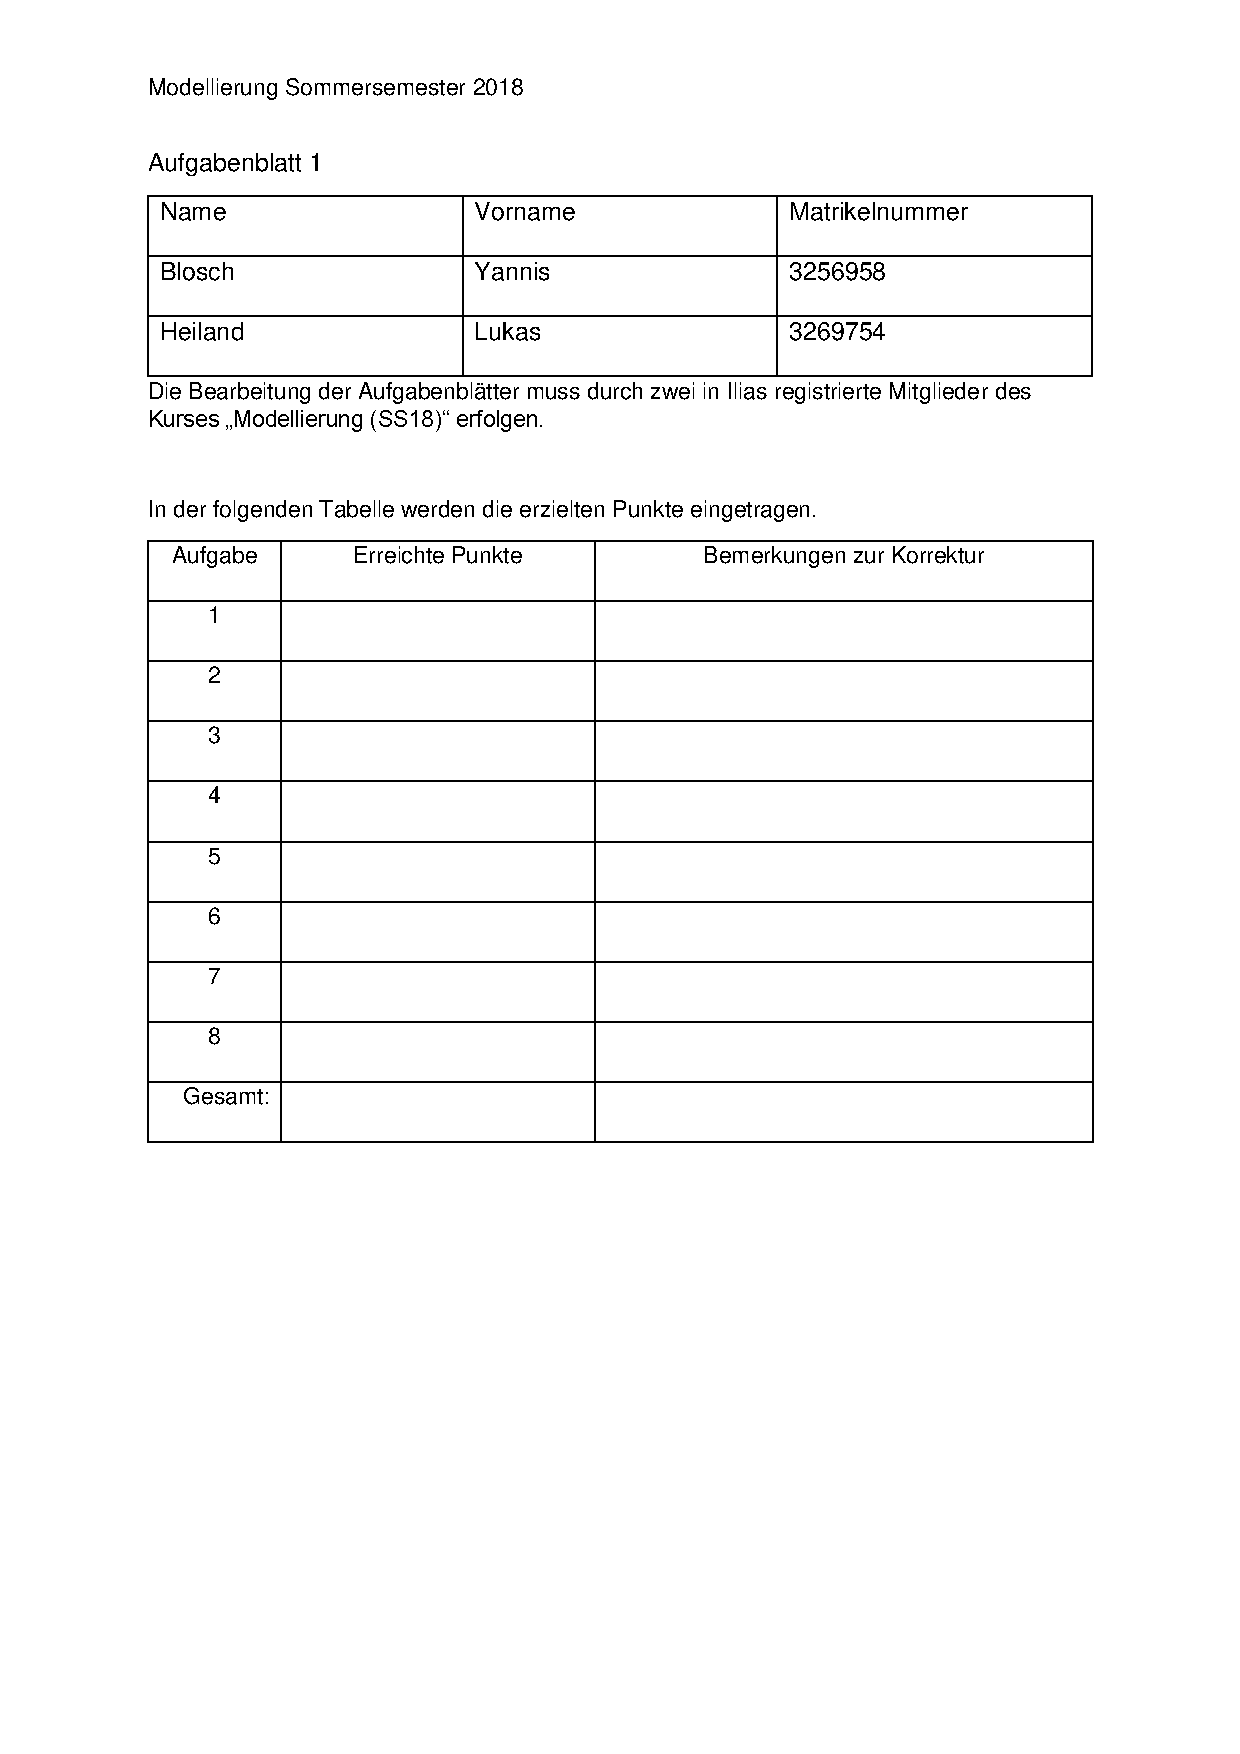
\includepdf{deckblatt.pdf}
	
	%%% format and header %%%
	% Counter für das Blatt und die Aufgabennummer.
% Ersetze die Nummer des Übungsblattes und die Nummer der Aufgabe
% den Anforderungen entsprechend.
% Beachte:
% \setcounter{countername}{number}: Legt den Wert des Counters fest
% \stepcounter{countername}: Erhöht den Wert des Counters um 1.
\newcounter{sheetnr}
\setcounter{sheetnr}{1} % Nummer des Übungsblattes
\newcounter{exnum}
\setcounter{exnum}{1} % Nummer der Aufgabe

% Befehl für die Aufgabentitel
\newcommand{\exercise}[1]{\section*{Aufgabe \theexnum\stepcounter{exnum} #1}} % Befehl für Aufgabentitel

% Formatierung der Kopfzeile
% \ohead: Setzt rechten Teil der Kopfzeile mit
% Namen und Matrikelnummern aller Bearbeiter
\ohead{Yannis Blosch (3256958)\\
Lukas Heiland (3269754)}
% \chead{} kann mittleren Kopfzeilen Teil sezten
% \ihead: Setzt linken Teil der Kopfzeile mit
% Modulnamen, Semester und Übungsblattnummer
\ihead{Modellierung\\
Sommersemester 2018\\
Blatt \thesheetnr}
	
	%%%%%%%%%%%%%%%%%%%%%%%%%%%%%%
	%%%%%%% actual content %%%%%%%
	%%%%%%%%%%%%%%%%%%%%%%%%%%%%%%
	
	
	% Aufgabe 3.1 %	
	\section*{Aufgabe 3.1}
	% always using .\\ to let the query begin on a new line
		\paragraph*{a}.\\
			\textbf{SELECT} *\\
			\textbf{FROM} abteilung\\
			\textbf{WHERE} ORT $=$ 'Dresden'
			\textbf{ORDER BY} ABTEILUNGSNR \textbf{DESC}
			
		\paragraph*{b}.\\
			\textbf{SELECT DISTINCT} angestellter.PERSONALNR,angestellter.WOHNORT,projekt.PROJEKTORT,abteilung.ORT\\
			\textbf{FROM} angestellter,projekt,projektmitarbeit,abteilung\\
			\textbf{WHERE} (angestellter.PERSONALNR = projektmitarbeit.PERSONALNR) \textbf{AND} (projekt.PROJEKTORT = angestellter.WOHNORT)\\ \textbf{AND} (angestellter.ABTEILUNGSNR = abteilung.ABTEILUNGSNR)
			
		\paragraph*{c}.\\
			\textbf{SELECT} ORT, \textbf{COUNT(*) as} Anzahl\\
			\textbf{FROM} abteilung\\
			\textbf{GROUP BY} ORT\\
			\textbf{HAVING COUNT(*)} > 1
			
		\paragraph*{d}.\\
			\textbf{SELECT} abteilung.ABTEILUNGSNR, \textbf{MAX}(angestellter.GEHALT) \textbf{as} Gehaltsmaximum\\
			\textbf{FROM} abteilung, angestellter\\
			\textbf{WHERE} abteilung.ABTEILUNGSNR $ = $ angestellter.ABTEILUNGSNR\\
			\textbf{GROUP BY} abteilung.ABTEILUNGSNR\\
			\textbf{HAVING} COUNT(angestellter.ABTEILUNGSNR) > 10
			
		
		% TODO YBL: e),f),g),h)
		
		
		% TODO TOGETHER: i) & j)
			
	
	% Aufgabe 3.2 %
	\section*{Aufgabe 3.2}
		\paragraph*{a.}
		
		\paragraph*{b.}.\\
			% ich glaub das ist richtig:
			% \textbf{DELETE}\\
			% \textbf{FROM} abteilung
			% \textbf{WHERE} ORT = Köln
			
		\paragraph*{c.}
		
		
		\paragraph*{d.}.\\
			\textbf{CREATE VIEW}  projects\_munich \textbf{AS}\\
			\textbf{SELECT} projekt.PROJEKTNR,projekt.PROJEKTNAME,projekt.PROJEKTORT\\
			\textbf{FROM} angestellter, projekt, projektmitarbeit\\
			\textbf{WHERE} angestellter.PERSONALNR = projektmitarbeit.PERSONALNR \textbf{AND} projektmitarbeit.PROJEKTNR = projekt.PROJEKTNR \textbf{AND} projekt.PROJEKTORT = 'Muenchen'\\
			\textbf{GROUP BY} projekt.PROJEKTORT, projekt.PROJEKTNAME,projekt.PROJEKTNR\\
			\textbf{HAVING} COUNT(*) >= 5
			
		\paragraph*{e.}.\\
			\textbf{DELETE FROM} projekt
		
		\pagebreak
			
		\paragraph*{f.}.\\
			\textbf{CREATE TABLE} angestellter(\\
			
				PERSONALNR integer \textbf{NOT NULL PRIMARY KEY},\\
				
				NAME varchar(25),\\
				
				VORNAME varchar(25),\\
				
				BERUF varchar(25),\\
				
				GEHALT decimal,\\
				
				ABTEILUNGSNR integer \textbf{FOREIGN KEY REFERENCES} abteilung(ABTEILUNGSNR) \textbf{NOTNULL},\\
				
				MANAGER integer \textbf{FOREIGN KEY REFERENCES} angestellter(PERSONALNR),\\
				
				GEBURTSTAG date,\\
				
				WOHNORT varchar(25));
			
			
\end{document}